\documentclass[10pt, oneside]{article}
\usepackage[utf8]{inputenc}
\usepackage{graphicx} % Required for inserting images
\usepackage{amsmath}
\usepackage{amssymb}
\usepackage[a4paper,left=2.1cm, right=2.1cm, top=2cm, bottom=2cm]{geometry}
\usepackage{verbatim}
\usepackage[english]{babel}
\usepackage{hyperref}
\usepackage{tikz}
\usetikzlibrary{decorations.pathreplacing,calligraphy}
\usetikzlibrary { decorations.pathmorphing, decorations.shapes, }
\usepackage[cal=dutchcal]{mathalfa}
\usepackage{wrapfig}
\usepackage{physics}
\usepackage{listings}
\usepackage{comment}
\renewcommand{\rmdefault}{cmss}

\lstdefinestyle{mystyle}{	basicstyle=\ttfamily\footnotesize
}

\lstset{style=mystyle}

\title{M.Sioli's Thermodynamics}
\author{Pocket reference for 1st year course - BSc Physics, Unibo}
\date{2023}

\begin{document}

\maketitle

\tableofcontents

\section{Fluidostatica e fluidodinamica}
\begin{description}
\item[Sforzo di Taglio] $\displaystyle \vec{T} = \frac{\mathrm{d}^{•} \vec{F}_t}{\mathrm{d}S^{•}}$
\item[Equazione della statica (1D)] $\displaystyle \frac{\mathrm{d}^{•} p}{\mathrm{d}z^{•}} = - \rho (z) g$
\item[Equazione generalizzata della statica] $\displaystyle \nabla p = \rho \vec{H} = - \rho \nabla \Phi$ ove $\vec{H}$ indica forza di volume (f. che agisce tramite il v. del corpo)
\item[Legge di Stevino] $p = p_0 + \rho g h$
\item[Tensione superficiale] $\displaystyle \tau = \frac{\mathrm{d}^{•} F}{\mathrm{d}l^{•}} = \frac{\mathrm{d}^{•} L}{\mathrm{d}S^{•}}$ (alternativamente indicata con $\gamma$)
\item[Equazione di continuità] $\rho A v = cost$
\item[Resistenza del mezzo (per corpo sferico)] $\displaystyle F = 6 \pi R \eta v$ a \textbf{piccole velocità}, $\displaystyle F = \frac{1}{2} \rho v^2 \cdot S \cdot C$ a \textbf{grandi v.}
\end{description}

\section{Sistemi termodinamici}
\begin{description}
\item[Regola delle Fasi di Gibbs] $\displaystyle \nu = C + 2 - F$ ove $\nu$ sono i d.o.f. termodinamici (var. intensive indipendenti), $C$ le componenti e $F$ le fasi
\item[Scala Celsius] $\displaystyle \theta (x) = 100 \frac{x - x_0}{x_{100} - x_0} \mathrm{°C}$
\item[Coefficiente di dilatazione termica lineare] $\displaystyle \alpha_L = \frac{1}{l} \bigg(\frac{\partial^{} l}{\partial T^{•}}\bigg)_p$ indicato anche con $\alpha$ \\(per un filo è a $\tau$, tensione ai capi, costante)
\\ $\boxed{\displaystyle \Delta l \approx l \cdot (1 + \alpha_L \Delta T)}$
\item[Coefficiente di dilatazione termica volumetrico] $\displaystyle \alpha =  \frac{1}{V} \bigg(\frac{\partial^{} V}{\partial T^{•}}\bigg)_p$ indicato anche con $\beta$
\\ $\boxed{\displaystyle \Delta V \approx V \cdot (1 + \alpha \Delta T)}$ Per $\Delta T \rightarrow 0$ $\beta \approx 3 \alpha_l$
\item[Coefficiente di comprimibilità isoterma] $\displaystyle \frac{1}{k} = -  \frac{1}{V} \bigg(\frac{\partial^{}V}{\partial p^{•}}\bigg)_T$
\item[Pendolo dilatato] anticipa in un giorno di $\Delta \tau_1$ a $\theta_1$ e $\Delta \tau_2$ a $\theta_2$
\[\alpha_L = \frac{2 (\Delta \tau_1 - \Delta \tau_2)}{\tau_0 (T_1 - T_2)}\]
\item[Potenziale di Lennard-Jones] $\displaystyle U(r) = \varepsilon \bigg[\bigg(\frac{r_{min}}{r}\bigg)^{12} - 2 \bigg(\frac{r_{min}}{r}\bigg)^6\bigg]$
\item[Termometro a GP] $\displaystyle \theta(p) = 273.16 \frac{p}{p_3}$ ove $p_3$ = punto triplo
\end{description}
\framebox{
\parbox{\linewidth}{
\textbf{LEGGI DEI GAS PERFETTI}
\begin{description}
\item[I Legge di Gay-Lussac] a $p$ cost $\displaystyle V = V_0 \beta \theta$ ($V \propto \theta$)
\item[II Legge di Gay-Lussac] a $V$ cost $\displaystyle p = p_0 \beta \theta$ ($p \propto \theta$)
\item[Legge di Boyle] a $n, \theta$ cost $\displaystyle V = \frac{cost}{p}$ ($\displaystyle V \propto \frac{1}{p}$)
\item[Legge di Avogadro] a $p, \theta$ cost $\displaystyle V = cost' \cdot n$ ($V \propto n$)
\item[Equazione di stato dei GP] $\boxed{\displaystyle pV = nR \theta}$
\end{description}
}
}

\begin{description}
\item[Dilatazione volumica e comprimibilità per GP] $\displaystyle \alpha = \frac{1}{\theta}$ \bigg| $k = p$ 
\item[Dipendenza pressione dalla quota ($\mathbf{\theta}$ cost)] $\displaystyle p(z) = p_0 \, e^{- z/h_0}$ con $\displaystyle h_0 = \frac{R \theta}{g \mathrm{M}}$ (massa molecolare media)
\item[Sviluppo del viriale] $\displaystyle z = \frac{pV}{nR\theta}$ fattore di compressione
\[z(p) \approx 1 + A p + B p^2 + C p^3 + ...\]
\item[Equazione di stato di Van der Waals] $\boxed{\displaystyle \big(p + a \frac{n^2}{V^2}\big) (V - bn) = nR\theta}$ 
\\oppure $\displaystyle \big(p + \frac{a}{\mathrm{v}^2}\big) (\mathrm{v} - b) = R \theta$ con volume molare $\mathrm{v}$
\item[Pressione per GR] $\displaystyle p(\theta, V) = \frac{nR\theta}{V - bn} - \frac{an^2}{V^2} = \frac{R\theta}{\mathrm{v} - b} - \frac{a}{\mathrm{v}^2} = p(\theta, \mathrm{v})$
\item[Temperatura e volume molare critici] (flesso orizzontale isoterma piano $p \mathrm{v}$) con coeff. compressione
\[\mathrm{v}_C = 3 b \quad \theta_C = \frac{8 a}{27 R b} \quad z_C = \frac{p_C \mathrm{v_C}}{R \theta_C} = \frac{3}{8} = 0.375\]
\item[Vapore saturo] $\displaystyle \frac{n_L}{n_G} = \frac{\mathrm{v}_G - \mathrm{v}}{\mathrm{v} - \mathrm{v}_L}$
\item[Recipienti comunicanti: si scalda 2] $\displaystyle p_f = \frac{V_1 + V_2}{V_1 + \frac{\theta_0}{\theta_f} V_2}$
\end{description}

\section{Teoria Cinetica}
\begin{description}
\item[Pressione] $\displaystyle p = \frac{1}{3} (p_x + p_y + p_z) = \frac{m}{3V} \sum\limits_{i=1}^N (v_{ix}^2 + v_{iy}^2 + v_{iz}^2) = \frac{m}{3V} \sum\limits_{i=1}^N v_i^2$
\item[Energia cinetica media] $\boxed{\displaystyle \langle \varepsilon \rangle = \frac{3}{2} k_B \theta}$
\item[Teorema di equipartizione dell'energia] definizione Kelvin $\displaystyle \theta = \frac{2 \langle \varepsilon \rangle }{k_B \nu}$ con $\nu  = n° \, d.o.f.$ e cost. di Boltzmann definita come valore esatto
\item[Legge di Dalton (pressioni parziali)] $\boxed{\displaystyle (p_1 + p_2) V = (n_1 + n_2) R \theta}$ \\ove $p_1, \, p_2$ sono pressioni esercitate in assenza dell'altro gas
\item[Gas sulla bilancia] $\displaystyle |\Delta v_{iy}| = \frac{gL}{|\vec{v}_{iy}|}$ da cui $\displaystyle \Delta p = \frac{Mg}{S}$
\item[Distribuzione di Boltzmann] (PDF) $\boxed{\displaystyle \rho (v; m, \theta) = \frac{4}{\sqrt{\pi}} \big(\frac{m}{2k_B \theta}\big)^{\frac{3}{2}} v^2 e^{\displaystyle - \frac{mv^2}{2k_B \theta}}}$ con $m$ massa della singola molecola
\item[Moda] $\displaystyle \frac{\mathrm{d}^{•} \rho}{\mathrm{d}v^{}} = 0$ $\rightarrow$ $\displaystyle \sqrt{\frac{2 R \theta}{M}} = \sqrt{\frac{2 k_B \theta}{m}}$
\item[Velocità media] $\displaystyle \langle v \rangle = \int_{0}^{+\infty}v \, \rho(v) \mathrm{d}v = \sqrt{\frac{8 R \theta}{\pi M}} = \sqrt{\frac{8 k_B \theta}{\pi m}}$
\item[Velocità quadratica media] \hfill $\displaystyle \langle v^2 \rangle = \int_{0}^{+\infty}v^2 \, \rho(v) \mathrm{d}v = \frac{3 R \theta}{M} = \frac{3 k_B \theta}{m}$ \hfill \bigg\rangle \hfill $\displaystyle \sqrt{\langle v^2 \rangle} = \sqrt{\frac{3 k_B \theta}{m}} = \sqrt{\frac{3 \pi}{8}} \langle v \rangle$ \hfill 
\item[Selettore di velocità] $\displaystyle \Delta l(v) = \frac{2 R^2 \omega}{v}$
\item[Atmosfere planetarie] raggio limite (posta $v_f = \sqrt{\langle v^2 \rangle}$) $\displaystyle r = \sqrt{\frac{9 R \theta}{8 G \pi M \rho_{pianeta}}}$ a $\theta, \rho$ unif
\item[Libero cammino medio - Mean free path] $\displaystyle \lambda = \frac{k_B \theta}{\sigma p \sqrt{2}}$ con $\sigma$ cross section molecole
\\\textbf{Frequenza urti} $\displaystyle f = \frac{\overline{v}}{\lambda} = \sqrt{\frac{6 \sigma p}{m k T}}$ \textbf{N° urti in unità di volume e tempo} $\displaystyle \mathcal{N}(V, \Delta t) = f \cdot \frac{N}{V} \cdot \Delta t = f \cdot \frac{p}{k T} \cdot \Delta t$
\end{description}

\section{Primo principio}
\begin{description}
\item[Lavoro] $\displaystyle L_{term} = \sum F_{GEN} \cdot \Delta S_{GEN}$ (tra sistema e ambiente, esterno)
\item[pV per quasistatiche] $\displaystyle \delta L = p \mathrm{d}V$ $\rightarrow$ $\displaystyle L = \int_{V_i}^{V_f}p(V)\mathrm{d}V$
\item[Altri tipi di lavori termodinamici] $\displaystyle L = \int_{i}^{f}p\mathrm{d}V + \int_{i}^{f}T \mathrm{d}l + \int_{i}^{f}\tau \mathrm{d}S + \int_{i}^{f}\varepsilon \mathrm{d}q + \int_{i}^{f}\mu_i \mathrm{d}n_i$
\item[\large LAVORO IN QUASISTATICHE]
\item[Isocora] $\displaystyle L = 0$
\item[Isobara] $\displaystyle L = p(V_f - V_i) = p \Delta V$
\item[Isoterma] per \textbf{GP} $\displaystyle L = nR \theta \ln \big(\frac{V_f}{V_i}\big)$ per \textbf{GR} $\displaystyle L = nR\theta \ln \bigg(\frac{V_f - nb}{V_i - nb}\bigg) + an^2 \big(\frac{1}{V_f} - \frac{1}{V_i}\big)$
\item[Per stati condensati] con dilatazione termica trasc: quasistatica $\displaystyle L = \frac{V}{k}[p_i^2 - p_f^2]$ brusca $\displaystyle L = - \frac{V}{k} p_f(p_f - p_i)$
\item[Bolla di sapone] differenza di pressione int-est $\displaystyle \Delta p = \frac{4 \tau}{r}$ 
\item[\large ENERGIA INTERNA E CALORE]
\item[En. interna e adiabatiche] $\displaystyle \Delta U_{A \rightarrow B} = L^{(ad)}_{A \rightarrow B}$
\item[PRIMO PRINCIPIO] integrale $\boxed{\displaystyle Q = \Delta U + L}$ locale $\boxed{\displaystyle \delta Q = \mathrm{d}U + \delta L}$
\\Convenzione segni:
\begin{center}
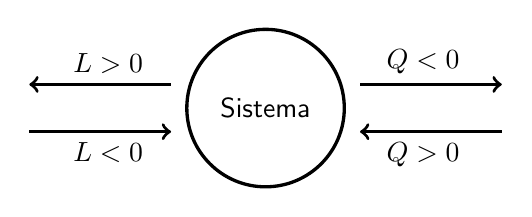
\begin{tikzpicture}

\filldraw[color=black, fill=white, very thick] (0,0) circle (1) node[anchor=center]{Sistema} ;

\draw[very thick, <-] (-3, 0.3) -- (-2, 0.3) node[anchor=south]{$L > 0$} -- (-1.2,0.3);
\draw[very thick, ->] (-3, -0.3) -- (-2, -0.3) node[anchor=north]{$L < 0$} -- (-1.2,-0.3);
\draw[very thick, <-] (3, 0.3) -- (2, 0.3) node[anchor=south]{$Q < 0$} -- (1.2,0.3);
\draw[very thick, ->] (3, -0.3) -- (2, -0.3) node[anchor=north]{$Q > 0$} -- (1.2,-0.3);
\end{tikzpicture}
\end{center}
\item[Sistemi idrostatici] semplici $\delta Q = p \mathrm{d}V + \mathrm{d}U$ non semplici $\delta Q = \sum p_i \mathrm{d}V_i + \mathrm{d}U$
\item[Altre forme di energia] sistema \textit{nella sua totalità} non in quiete $\boxed{\displaystyle + \Delta K}$ e/o sottoposto a campo di forze, potenziale conservativo $\boxed{\displaystyle + \Delta V}$
\item[Ciclo] $\Delta U = 0$ $\implies$ $Q = L$
\item[\large CAPACIT\'A TERMICA]
\item[C.t. media] $\displaystyle \overline{C} = \frac{Q}{\Delta T}$
\item[Locale] $\displaystyle C(\theta) = \lim\limits_{\theta_f \rightarrow \theta}\frac{Q}{\theta_f - \theta} = \frac{\delta Q}{\mathrm{d}\theta}$
\item[Calore specifico] $\displaystyle c_m = \frac{C}{m} = \frac{1}{m} \frac{\delta Q}{\mathrm{d}\theta}$ \bigg| $[c_m] = \mathrm{J \, K^{-1} \, kg^{-1}}$
\item[Calore molare] $\displaystyle \mathcal{c}_n = \mathcal{c} = \frac{C}{n}$ \bigg| $[\mathcal{c}] = \mathrm{J \, K^{-1} \, mol^{-1}}$
\\A pressione costante $\displaystyle \mathcal{c}_p = \frac{1}{n} \bigg(\frac{\delta Q}{\mathrm{d}\theta}\bigg)_p$, a volume costante $\displaystyle \mathcal{c}_V = \frac{1}{n} \bigg(\frac{\delta Q}{\mathrm{d}\theta}\bigg)_V$
\item[Calore latente] locale $\displaystyle \lambda = \frac{\delta Q}{\mathrm{d}m}$, integrale $\displaystyle \lambda = \frac{Q}{m}$ con $m$ massa che transisce di fase e $Q$ assorbito o ceduto. \\Anche molare $\displaystyle \lambda_n = \frac{Q}{n}$
\item[Lungo politropica per GP] $\displaystyle p V^\alpha = cost$ $\implies$ $\displaystyle \mathcal{c}_\alpha = \mathcal{c}_V + \frac{R}{1-\alpha}$ (si riduce a $\displaystyle \mathcal{c}_p$ se $\alpha = 0$)
\item[Lavoro in transizione] e.g. liquido-vapore $\displaystyle L = p(\mathrm{v}_G - \mathrm{v}_L)$
\item[Dulong-Petit e Debye] $\displaystyle \mathcal{c} \approx \mathcal{c}_V(\theta)=3R\big(\frac{\theta}{\theta_D}\big)^3\int_{0}^{\theta_D/\theta}\frac{x^4 e^x}{(e^x-1)^2}dx$ 
\\per $\displaystyle \theta \gg \theta_D$ $\longrightarrow$ $\mathcal{c} \approx 3 R$ cost
\\per $\displaystyle \theta \ll \theta_D$ $\longrightarrow$ $\displaystyle \mathcal{c} \propto \big(\frac{\theta}{\theta_D}\big)^3$
\item[GP]\textbf{Monoatomici} $\displaystyle \mathcal{c}_V = \frac{3}{2}R$ \bigg| $\displaystyle \mathcal{c}_p = \frac{5}{2} R$ \bigg| $\displaystyle \gamma = \frac{5}{3}$
\\\textbf{Biatomici} 
$\displaystyle \mathcal{c}_V = \frac{5}{2}R$ \bigg| $\displaystyle \mathcal{c}_p = \frac{7}{2} R$ \bigg| $\displaystyle \gamma = \frac{7}{5}$
\item[Calorimetro di Bunsen] $\displaystyle c_m = \frac{\lambda_f}{m_c \Delta \theta} \frac{\Delta V}{\Delta V_{LS}} = \frac{\lambda_f m_G}{m_c \Delta \theta}$ ove $\Delta V_{LS}$ è la variazione di vol. per unità di massa sciolta
\item[Equilibrio termico] $\displaystyle \theta_e = \frac{C_1 \theta_1 + C_2 \theta_2}{C_1 + C_2}$ per termostato $\displaystyle \theta_e = \frac{\displaystyle 1 + \frac{C_2}{C_1} \frac{\theta_2}{\theta_1}}{\displaystyle 1 + \frac{C_2}{C_1}} \theta_1 \xrightarrow[\displaystyle \frac{C_2}{C_1} \rightarrow 0]{} \theta_1$
\item[Calorimetro delle mescolanze (di Regnault)] $\displaystyle c = c_{H_2O} \frac{m_{H_2O}}{m}\bigg[\frac{\theta_e - \theta_{H_2O}}{\theta - \theta_e}\bigg]$ con $\displaystyle m_{H_2O} = m_{H_2O}^0 + m_{H_2O}^{(equiv)}$
\item[Calori molari per sistemi idrostatici]
$\displaystyle \mathcal{c}_V = \frac{1}{n} \bigg(\frac{\partial U}{\partial \theta}\bigg)_V$ \hfill \bigg| \hfill $\displaystyle \mathcal{c}_p = \frac{1}{n} \bigg[\bigg(\frac{\partial U}{\partial \theta}\bigg)_p + p \bigg(\frac{\partial V}{\partial \theta}\bigg)_p\bigg] = \frac{1}{n} \bigg(\frac{\partial H}{\partial \theta}\bigg)_p$ \\(vd. potenziali)
\item[Energia interna GP] $\boxed{\displaystyle \mathrm{d}U = n \mathcal{c}_V \mathrm{d}\theta}$ da cui assunto calore molare costante $\displaystyle U(\theta) = n \mathcal{c}_V \theta + cost$
\end{description} 
\begin{center}
\begin{tikzpicture}

\draw[thick, ->] (-3,0) -- (-1.5,0)node[anchor=north]{$V_i$} -- (0,0) node[anchor=north]{$2V_i$} -- (1,0) node[anchor=north]{$V$};

\draw[thick, ->] (-3,0) -- (-3,1)node[anchor=east]{$p_i/2$} -- (-3,2)node[anchor=east]{$p_i$} -- (-3,4) node[anchor=east]{$p$};

\draw[thick, dashed] (-3,2) -- (-1.5, 2) -- (-1.5, 0);
\draw[thick, dashed] (-3, 1) -- (0,1) -- (0,0);

\draw[very thick] (-1.5,2) -- (-0.75,1.5)node[anchor=west]{$\quad \displaystyle \mathcal{c}_\tau (V) = R \frac{15 - 8 V/V_i}{6 - 4 V/V_i}$}  -- (0,1);
\draw[very thick, ->] (-1.5, 2) -- (-0.75, 1.5);
\end{tikzpicture}
\end{center}
\begin{description}
\item[Seconda equazione dell'energia] $\displaystyle \bigg(\frac{\partial U}{\partial V}\bigg)_\theta = \theta \bigg(\frac{\partial p}{\partial \theta}\bigg)_V - p$
\item[Energia interna GR] $\displaystyle U(\theta, V) = n \mathcal{c}_v \theta - \frac{a n^2}{V} + cost$ 
\item[TEOREMA DI EQUIPARTIZIONE (bis)] $\displaystyle \mathcal{c}_V = \frac{f}{2} R$ con $f$ d.o.f.
\item[Contributi cinetici (K\"onig)] $\displaystyle \varepsilon = \varepsilon_{TRASL} + \varepsilon_{ROT} + \varepsilon_{VIBR}$ per quest'ultima 2 termini per ogni modo vibrazionale
\item[Biatomici] $f = $ 3 trasl + 2 rot (terzo asse princ d'inerzia trasc) + 2 vib (attivi solo sopra alta soglia quantica)
\item[Poliatomici] $f =$ 3 trasl + $\displaystyle \overbrace{f_{ROT}^{ANG} = 3 \, \lor \, f_{ROT}^{LIN} =2}$ + $\displaystyle  \overbrace{f_{VIB}^{ANG} = 2(3N - 6) \, \lor \, f_{VIB}^{LIN} = 2(3N - 5)}$
\\dunque $\displaystyle \mathcal{c}_V^{ANG} = 3R (N-1)$ \bigg| $\displaystyle \mathcal{c}_V^{LIN} = \frac{6N - 5}{2}R$
\item[Relazione di Meyer (per GP)] $\boxed{\displaystyle \mathcal{c}_p = \mathcal{c}_V + R}$
\item[$\mathbf{\gamma}$ per poliatomici] $\displaystyle \gamma_{LIN} = 1 + \frac{2}{6N - 5}$ \bigg| $\displaystyle \gamma_{ANG} = 1 + \frac{1}{3N -3}$ \\(ma nel limite di $N$ elevato correzioni quantistiche non trascurabili!)
\item[Adiabatiche di sistemi idrostatici] $\displaystyle \gamma \frac{\mathrm{d}V}{V} = - \frac{\mathrm{d}p}{p}$ $\rightarrow$ $\displaystyle pV^\gamma = cost$ \bigg| $\displaystyle \theta V^{\gamma - 1} = cost$ \bigg| $\displaystyle \theta p^{ \frac{1 - \gamma}{\gamma}} = cost$
\item[Lavoro in QS per GP]$\displaystyle L = \frac{p_i V_i - p_f V_f}{\gamma - 1} = \delta U$
\item[Curve] $\displaystyle \bigg(\frac{\partial p}{\partial V}\bigg)_T = - \frac{p}{V} > \bigg(\frac{\partial p}{\partial V}\bigg)_{ad} = - \gamma \frac{p}{V}$ $\implies \enspace \bigg|\bigg(\displaystyle \frac{\partial p}{\partial V}\bigg)_T\bigg| < \bigg|\bigg(\displaystyle \frac{\partial p}{\partial V}\bigg)_{ad}\bigg|$ (adiabatica più 'ripida')
\end{description}

\begin{minipage}{0.3\textwidth}
\centering
\vspace{-0.3cm}
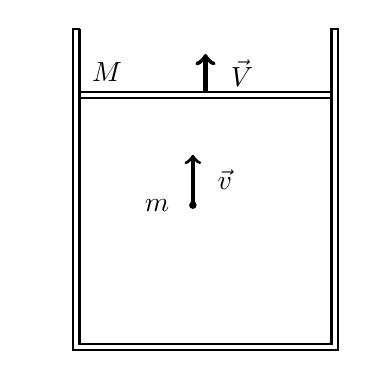
\begin{tikzpicture}[scale=0.8]
\draw[thick] (-2,5) -- (-2,0) -- (2,0) -- (2,5) -- (2.1, 5) -- (2.1, -0.1) -- (-2.1, -0.1) -- (-2.1, 5) -- (-2,5);
\draw[thick] (-2,4)node[anchor=south]{$\quad \quad M$} -- (2,4) -- (2,3.9) -- (-2, 3.9);

\draw[ultra thick, ->] (0,4) -- (0,4.3) node[anchor=west]{$\enspace \vec{V}$} -- (0, 4.6);

\filldraw[color=black] (-0.2, 2.2) circle(0.05) node[anchor=east]{$m \enspace$};
\draw[very thick, ->] (-0.2, 2.2) -- (-0.2, 2.6)node[anchor=west]{$\enspace \vec{v}$} --  (-0.2, 3);
\end{tikzpicture}
\end{minipage}
\begin{minipage}{0.7\textwidth}
\begin{description}
\item[Spiegazione meccanica per esp adiabatica] $\displaystyle r \equiv \frac{m}{M}$
\\$\displaystyle V' = \frac{2m v + (M - m) V}{m+M} \xrightarrow[r \rightarrow 0]{} V$ (immutato) \\$\displaystyle v' = \frac{2M V + (m-M)v}{m+M} \xrightarrow[r \rightarrow 0]{} 2V - v$ (varia modulo: si ha mediamente diminuzione $\varepsilon$ e dunque $\Delta U, \, \Delta \theta < 0$)
\item[Prima equazione di Friedmann - espansione adiabatica dell'universo]
\[ \dot \rho = -3(p + \rho)H\] con $\displaystyle H = \frac{\dot a}{a}$ costante di Hubble
\end{description}
\end{minipage}

\begin{description}
\item[Dipendenza temperatura dalla quota] $\displaystyle L \equiv \frac{\gamma - 1}{\gamma} \frac{\mathcal{M} g}{R}$ Lapse rate (gradiente adiabatico secco) $\displaystyle \frac{\mathrm{d}^{•} \theta}{\mathrm{d}z^{•}} = -L \implies \theta(z) = \theta_0 - Lz$ (in realtà si usa lapse rate umido - o saturo)
\item[Dipendenza pressione]$\displaystyle \frac{\mathrm{d}^{•} p}{p} = \frac{\mathcal{M}g}{RL}\frac{L \mathrm{d}z}{\theta_0 - Lz}$ $\implies \enspace p(z) = p_0 \bigg(\displaystyle 1 - \frac{Lz}{\theta_0}\bigg)^{\displaystyle \frac{\mathcal{M}g}{RL}}$
\item[Esperienza di R\"uchardt] $\displaystyle \gamma = \frac{4 \pi^2 mV}{A^2 p \tau}$ ove $\tau$ = periodo di oscillazione, $A$ sezione tubo
\item[Velocità del suono]$\displaystyle v = \sqrt{\frac{k_s}{\rho}}$ con $\displaystyle k_S = \bigg[-\frac{1}{V} \bigg(\frac{\partial V}{\partial p}\bigg)_S\bigg]^{-1}$ coeff. di comprimibilità adiabatico
\\si ottiene $\boxed{\displaystyle \gamma = \frac{v^2 \rho}{p}}$
\item[Curva generica nel piano pV] Massimizz $T$ $\rightarrow$ si ricava $p(V)$ e sostituisce in eq. di stato $\rangle$ $\displaystyle \bigg(\frac{\partial T}{\partial V}\bigg)_\tau = 0$ per $V_{max}$
\item[Velocità angolare media biatom] $\displaystyle \langle \varepsilon_{ROT} \rangle = \langle \frac{1}{2} I_A \omega_A^2 + \frac{1}{2} I_B \omega_B^2 \rangle = \frac{2}{2} k T = k T$ \hfill \bigg\rangle \hfill $\displaystyle \langle \omega^2 \rangle = 2 \cdot \langle \omega_i^2 \rangle = \frac{2 k T}{m d^2}$ \\con $m = m_{nucleo}$ e $d = d_{legame}$
\item[Radiazione elettromagnetica] $\approx$ gas di fotoni \hfill \big\rangle \hfill $\displaystyle U = b V T^4$ \hfill \big| \hfill $\displaystyle p = \frac{1}{3} b  T^4$ \hfill \big\langle \hfill $\displaystyle b = 7.56 \times 10^{-16} \mathrm{J \, K^{-4} \, m^{-3}}$
\\Espansione adiabatica dell'universo osservabile: $\displaystyle R_0 T_0 = R_f T_f$
\item[Pistone adiabatico con molla] elongazione quando accelerazione pistone eguaglia quella del contenitore:
\[\Delta l = \frac{m_{pist} \cdot a_{cont}}{\displaystyle k + \frac{8 \gamma V_0 p_0}{l^2}}\]
\item[Velocità massima setto mobile] adiabatico che divide due gas con stesso $\gamma$ in contenitore isolato
\[v_{max} = \sqrt{\frac{2}{m(1-\gamma)} \bigg[p_{eq}(V_{TOT}) - p_1^0 V_1^0 - p_2^0 V_2^0\bigg]}\]
\item[Capacità termica contenitore con pistone e molla] $\displaystyle C = \frac{Q}{\Delta T} = \frac{\Delta U}{\Delta T} = 2 R$ 
\item[Due camere: setto fisso conduttore + pistone mobile adiabatico] $\boxed{ B \, \bigg{\|} \, A \leftarrow \bigg| \rightarrow }$ \\ \[L_e = - \frac{3}{2} R (T_f -T_0) (n_B + n_A) \quad \bigg| \quad p_B^f = \frac{n_A \, R \, T_f}{V_A} \quad \bigg| \quad \textrm{ politropica: } p V^{\frac{5n_A + 3n_B}{3 n_A + 3 n_B}} = cost\]
\item[Adiabatico con aggiunta massa] $\displaystyle T_f = \frac{2}{5nR} \bigg(p_0 A + M g\bigg) (h_0 - h_f) + T_0$ \bigg/ $\displaystyle h_f = \bigg[1 - \frac{x}{\gamma (1 + x)}\bigg] h_0$ con $\displaystyle x \equiv \frac{M g}{p_0 A}$
\item[Vapor d'acqua e ghiaccio a 0°C] con vapore estratto: rimane solo ghiaccio $\Rightarrow$ $\displaystyle m_G = \frac{\lambda_V}{\lambda_V + \lambda_F} V_0 \rho_{H_2O}$
\end{description}

\section{Trasmissione del calore}
\begin{description}
\item[\large Conduzione: Legge di Fourier] 
\[\boxed{\frac{\delta Q}{\mathrm{d}t} = - k \, \mathrm{d}A \, \bigg(\frac{\mathrm{d}\theta}{\mathrm{d}x}\bigg)}\] ove l'ultimo termine indica il gradiente termico, $[k] = \mathrm{W m^{-1} K^{-1}}$ la conducibilità termica (segno negativo in quanto fluisce da più caldo a più freddo)
\[\underbrace{\vec{\Phi}_Q}_{\textrm{flusso di } Q} = - k \vec{\nabla} \theta\]
\item[Trattazione generale: equazione del trasporto] $\displaystyle \frac{\partial^{•} u}{\partial t^{•}} + \mathbf{b} \cdot \nabla u = f$ con $u \, : \, \mathbb{R}^n \times \mathbb{R}^+ \rightarrow \mathbb{R}$, $\mathbf{b} \, \in \, \mathbb{R}^n$
\item[Geometria planare] $\displaystyle P = \frac{\delta Q}{\mathrm{d} t} = k \cdot A \cdot \frac{\theta_1 - \theta_2}{d} = - A H \Delta \theta$ con \textbf{conduttanza} $\displaystyle H \equiv \frac{k}{d}$
\item[Conduttanza di strati in serie] $\displaystyle \frac{1}{H_{tot}} = \sum_i \frac{1}{H_i}$
\item[Caso non stazionario: equazione del calore] $\displaystyle \nabla^2 \theta = \frac{\rho c}{k} \frac{\partial^{•} \theta}{\partial t^{•}}$ con $\displaystyle \alpha \equiv \frac{\rho c}{k}$ diffusività termica
\item[Geometria cilindrica] $\displaystyle \frac{\delta Q}{\mathrm{d} t} = 2 \pi \cdot l \cdot k \frac{\theta_1 - \theta_2}{\displaystyle \ln \frac{r_2}{r_1}}$ con $1$ int, $2$ est
\item[Geometria sferica] $\displaystyle \frac{\delta Q}{\mathrm{d} t} = 4 \pi k \bigg(\frac{r_2 r_1}{r_1 - r_2}\bigg)(\theta_1 - \theta_2)$
\item[Superficie ghiacciata del lago / nel contenitore] spessore $\displaystyle z(t) = \sqrt{2 \bigg(\frac{k \dd{T}}{\lambda_f \rho_G	}\bigg) t + z_0^2}$
\end{description}
\begin{minipage}{0.6\textwidth}
\subsection*{Convezione: legge del raffreddamento di Newton}
\[\boxed{\frac{\delta Q}{\mathrm{d} t} = h \, \mathrm{d}A \,(\theta_0 - \theta_\infty)}\]
con $h$ coefficiente di trasferimento termico (o di convezione)
\begin{description}
\item[Raffreddamento del tè] $\displaystyle \theta(t) = (\theta_0 - \theta_\infty) \, e^{\displaystyle - \frac{hA}{C}t} + \theta_\infty$
\end{description}
\end{minipage}
\begin{minipage}{0.4\textwidth}
\vspace{0cm}
\centering
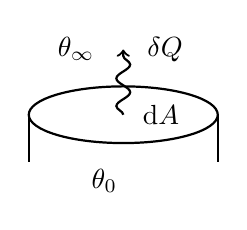
\begin{tikzpicture}[scale=1.2]
\draw[thick] (0,0) ellipse (1 and 0.3);
\draw[thick] (-1,0) -- (-1, -0.5);
\draw[thick] (1,0) -- (1,-0.5);
\node[draw opacity = 0] at (0.4,0){$\dd A$};
\draw[thick, decorate, decoration=snake, ->] (0,0) -- (0, 0.69)node[anchor=west]{$\enspace \delta Q$};
\node[draw opacity = 0] at (-0.5, 0.7){$\theta_\infty$};
\node[draw opacity = 0] at (-0.2, -0.7){$\theta_0$};
\end{tikzpicture}
\vfill
\end{minipage}

\begin{description}
\item[Tempo di raffreddamento] $\displaystyle \dv[•]{T}{t} = - \frac{h A}{V \rho c}(T - T_\infty)$ da cui $\displaystyle t_f = \frac{V \rho c}{h A} \ln \bigg( \frac{T_i - T_\infty}{T_f - T_\infty} \bigg)$
\end{description}
\subsection*{Irraggiamento: legge di Stefan-Boltzmann}
\[\boxed{\frac{\delta Q}{\mathrm{d}t} = \varepsilon \, \sigma \, A \, \theta^4}\]
con $0<\varepsilon<1$ approssimabilità a corpo nero, $\sigma$ cost. di S-B

\begin{description}
\item[Corpi irradiati] $\displaystyle \underbrace{r(\alpha, \lambda)}_{riflettanza} + \underbrace{a(\alpha, \lambda)}_{assorbanza} + \underbrace{t(\alpha, \lambda)}_{trasmittanza} = 1$ con $\alpha$ angolo di incidenza. Dopo assorbimento si ha emissione:
\item[Legge di Kirchhoff] emittanza $\displaystyle \epsilon(\lambda) = \int a(\lambda)$ sull'angolo solido (tutta riemessa)
\end{description}

\begin{minipage}{0.4\textwidth}
\centering
\vspace{-1cm}
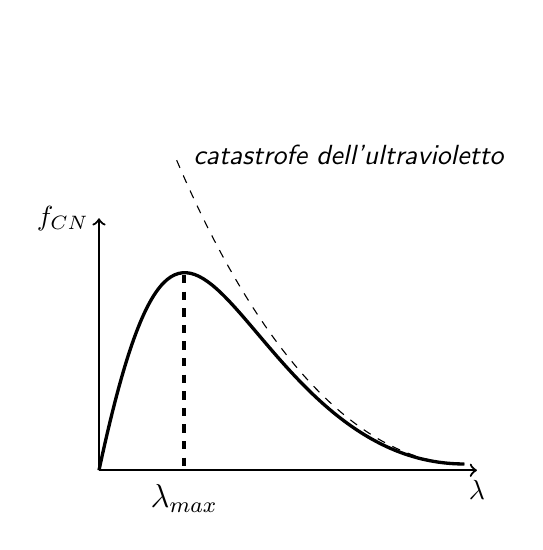
\begin{tikzpicture}[scale=0.8]
\draw[thick, ->] (-3,0) -- (3,0) node[anchor=north]{$\lambda$};

\draw[thick, ->] (-3,0) -- (-3,4) node[anchor=east]{$f_{CN}$};
\draw[very thick] (2.8, 0.1) .. controls (-0.9,0.1) and (-1.5, 7) .. (-3, 0);
\draw[dashed] (2.8, 0.1) .. controls (2,0.1) and (0.1, 0.5) .. (-1.8, 5)node[anchor=west]{{} \textit{catastrofe dell'ultravioletto}};
\draw[dashed, very thick] (-1.65, 3.1) -- (-1.65,-0.05)node[anchor=north]{\large $\lambda_{max}$};
\end{tikzpicture}
\end{minipage}
\begin{minipage}{0.6\textwidth}
\begin{description}
\item[Radiazione elettromagnetica] $\displaystyle \lambda \nu = c$ 
\\$\displaystyle E = h \nu$ con $h$ costante di Planck
\item[Spettro di Corpo Nero: Legge di Planck] (curva planckiana)
\[\boxed{f_{CN}(\lambda; \, \theta) = \frac{c_1}{\lambda^5 \big(\displaystyle e^{c_2 / \lambda \theta} - 1 \big)}}\]
$\displaystyle \int_{0}^{\infty}f_{CN}(\lambda) \mathrm{d}\lambda = \sigma \theta^4$ (energia totale per unità di tempo e superficie - flusso irradiato)
\end{description}
\end{minipage}
\begin{description}
\item[Legge di Wien] $\displaystyle \theta \, \lambda_{max} = cost = b$ costante dello spostamento di Wien (massimo si ottiene annullando derivata)
\end{description}
\textbf{Emittanza} monocromatica: $\displaystyle \epsilon^{(\lambda)} = \frac{f(\lambda)}{f_{CN}(\lambda)}$ (tra corpo in esame e CN). Parametro della legge si ottiene secondo:
\[\varepsilon = \frac{\int f(\lambda)\, \mathrm{d}\lambda}{\int f_{CN}(\lambda)\, \mathrm{d}\lambda}\]

\section{II Principio}
\begin{description}
\item[Kelvin-Planck] per cicli monotermi $\displaystyle Q = L \leq 0$
\item[Rendimento/efficienza macchina termica] $\boxed{\displaystyle \eta = \frac{L}{Q_{ass}} = 1 + \frac{Q_{ced}}{Q_{ass}} = 1 - \frac{|Q_{ced}|}{|Q_{ass}|}}$ \\ove $Q_{ass}$ e $Q_{ced}$ sono la somma dei calori ceduti ai ed assorbiti dai vari serbatoi (anche più di 2)
\end{description}
\vspace{-0.15cm}
\begin{minipage}{0.4\textwidth}
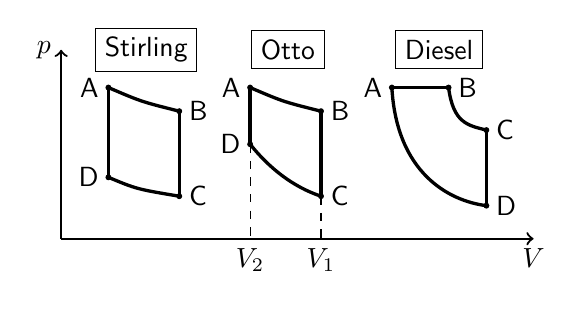
\begin{tikzpicture}[scale=0.6]
\draw[thick, ->] (-3,0) -- (7,0) node[anchor=north]{$V$};

\draw[thick, ->] (-3,0) -- (-3,4) node[anchor=east]{$p$};

\draw[very thick] (-2,1.3) -- (-2,3.2);
\draw[very thick] (-2, 3.2) .. controls (-1.3,2.9) .. (-0.5, 2.7);
\draw[very thick] (-0.5,2.7) -- (-0.5, 0.9);
\draw[very thick] (-2, 1.3) .. controls (-1.4,1.05) .. (-0.5, 0.9);
\filldraw[color=black] (-2,1.3) circle(0.05)node[anchor=east]{D};
\filldraw[color=black] (-2,3.2) circle(0.05)node[anchor=east]{A};
\filldraw[color=black] (-0.5,2.7) circle(0.05)node[anchor=west]{B};
\filldraw[color=black] (-0.5,0.9) circle(0.05)node[anchor=west]{C};
\node[draw] at (-1.2,4) {Stirling};

\draw[very thick] (1,2) -- (1,3.2);
\draw[very thick] (1, 3.2) .. controls (1.7,2.9) .. (2.5, 2.7);
\draw[very thick] (2.5,2.7) -- (2.5, 0.9);
\draw[very thick] (1, 2) .. controls (1.4,1.5) and (1.9, 1.1).. (2.5, 0.9);
\draw[dashed] (1,2) -- (1,0) node[anchor=north]{$V_2$};
\draw[dashed] (2.5,0.9) -- (2.5,0) node[anchor=north]{$V_1$};
\filldraw[color=black] (1,2) circle(0.05)node[anchor=east]{D};
\filldraw[color=black] (1,3.2) circle(0.05)node[anchor=east]{A};
\filldraw[color=black] (2.5,2.7) circle(0.05)node[anchor=west]{B};
\filldraw[color=black] (2.5,0.9) circle(0.05)node[anchor=west]{C};
\node[draw] at (1.8, 4) {Otto};

\draw[very thick] (4,3.2) -- (5.2,3.2);
\draw[very thick] (5.2, 3.2) .. controls (5.3,2.45) and (5.6, 2.4) .. (6, 2.3);
\draw[very thick] (6,2.3) -- (6, 0.7);
\draw[very thick] (4, 3.2) .. controls (4.1,1.4) and (5.2, 0.8) .. (6, 0.7);
\filldraw[color=black] (4,3.2) circle(0.05)node[anchor=east]{A};
\filldraw[color=black] (5.2,3.2) circle(0.05)node[anchor=west]{B};
\filldraw[color=black] (6,2.3) circle(0.05)node[anchor=west]{C};
\filldraw[color=black] (6,0.7) circle(0.05)node[anchor=west]{D};
\node[draw] at (5, 4) {Diesel};

\end{tikzpicture}
\hspace{1cm}
\end{minipage}
\begin{minipage}{0.6\textwidth}
\begin{description}
\item[Ciclo di Stirling] (combustione esterna) 
\\$\displaystyle \eta = \frac{R \ln \bigg(\displaystyle \frac{V_B}{V_A}\bigg) (\theta_1 - \theta_2)}{\displaystyle \theta_1 R\ln \bigg(\frac{V_B}{V_A}\bigg) + \mathcal{c}_V(\theta_1 - \theta_2)}$
\item[Ciclo Otto] (comb. interna) $\displaystyle \eta = 1 - \frac{1}{\bigg(\displaystyle \frac{V_1}{V_2}\bigg)^{\gamma -1}} = 1 - \bigg(\displaystyle \frac{V_2}{V_1}\bigg)^{\gamma -1}$
\item[Ciclo Diesel]
$\displaystyle \eta = 1 - \frac{\mathcal{c}_V}{\mathcal{c}_p} \frac{\theta_C - \theta_D}{\theta_B - \theta_A}$
\end{description}
\end{minipage}
\\
\begin{minipage}{0.4\textwidth}
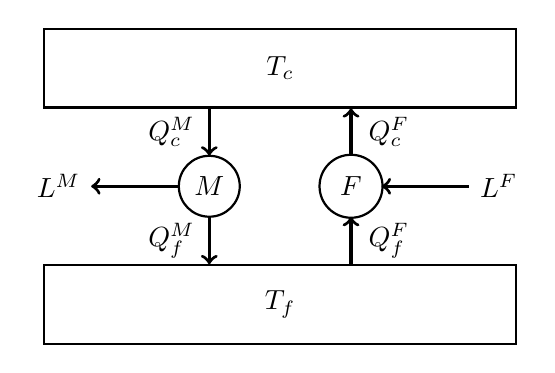
\begin{tikzpicture}[scale=0.3]
\node[rectangle, draw=black, thick, fill=white, minimum width = 6cm, minimum height = 1cm] at (0,10) {$T_c$};
\node[rectangle, draw=black, thick, fill=white, minimum width = 6cm, minimum height = 1cm] at (0,0) {$T_f$};
\node[circle, draw=black, thick, minimum size = 0.6cm] at (-3,5) {$M$};
\draw[very thick, <-] (-3,1.7) -- (-3, 3.7);
\node[draw opacity= 0] at (-4.6, 2.7) {$Q_f^M$};
\draw[very thick, <-] (-3,6.3) -- (-3, 8.3);
\node[draw opacity = 0] at (-4.6, 7.3) {$Q_c^M$};
\draw[very thick, ->] (-4.3, 5) -- (-8,5) node[anchor=east]{$L^M$};

\node[circle, draw=black, thick, minimum size = 0.8cm] at (3,5) {$F$};
\draw[very thick, ->] (3,1.7) -- (3, 3.7);
\node[draw opacity= 0] at (4.6, 2.7) {$Q_f^F$};
\draw[very thick, ->] (3,6.3) -- (3, 8.3);
\node[draw opacity = 0] at (4.6, 7.3) {$Q_c^F$};
\draw[very thick, <-] (4.3, 5) -- (8,5) node[anchor=west]{$L^F$};
\end{tikzpicture}
\end{minipage}
\begin{minipage}{0.6\textwidth}
\begin{description}
\item[Coefficiente di prestazione (macchina frigorifera)] { } \, { }
\\$\boxed{\displaystyle \varepsilon \, (\, \omega \, ) \, = \frac{Q_f}{|L|} = \frac{|Q_f|}{|Q_c| - |Q_f|}}$
\item[Teorema di Carnot] $\eta_M \leq \eta_C$ per MdC operante \textit{con} i medesimi serbatoi \textit{tra} o \textit{con} cui opera $M$. Uguaglianza se $M$ di Carnot
\end{description}

\end{minipage}

\begin{description}
\item[Rendimento MdC] $\boxed{\displaystyle \eta_C = 1 - \frac{T_f}{T_c}}$ \hfill \textbf{Coeff di prestazione frigo di Carnot} $\boxed{\displaystyle \omega_C = \frac{T_f}{T_c - T_f}}$
\item[Temperatura termodinamica assoluta] $\displaystyle T_x = T_3 \frac{|Q_x|}{|Q_3|}$ definita da rapporto calori scambiati da MdC che opera tra essa e il punto triplo.
\item[Massimo lavoro estraibile:] \textbf{Serbatoio caldo a $C < \infty$} : $\displaystyle L_{max} = C\bigg[T_c - T_f + T_f \ln \frac{T_f}{T_c}\bigg]$ \\ \textbf{Freddo a $C < \infty$} : $\displaystyle L_{max} = C \bigg[T_f - T_c + T_c \ln \frac{T_c}{T_f}\bigg]$
\item[MdC tra serbatoi a $C$ finita e costante] $\displaystyle C_c = C_f$ \hfill \big\rangle \hfill $\displaystyle T_e = \sqrt{T_c \cdot T_f}$ \hfill \big| \hfill $\displaystyle L = C (T_c + T_f - 2 T_e)$
\item[M irr \textit{tra} serbatoi accoppiata con $\mathbf{\overline{C}}$] definito $\displaystyle \epsilon = \frac{\displaystyle Q_c^M}{\displaystyle Q_c^{\overline{C}}}$ si ha $\displaystyle \eta_M = \frac{1}{\epsilon} \eta_C$ \hfill \big| \hfill $\displaystyle \Delta S_{ciclo} = \frac{Q_f^M}{T_f} \bigg[\bigg(\frac{T_c}{T_f} - 1\bigg)(\epsilon - 1)\bigg]$
\end{description}
\section{Entropia}
\begin{description}
\item[\large Teorema (o disuguaglianza) di Clausius] caso discreto $\boxed{\displaystyle \sum\limits_{i=1}^n \frac{Q_i}{T_i} \leq 0}$ al continuo $\boxed{\displaystyle \oint \frac{\delta Q}{T} \leq 0}$ ove $T$ è la temperatura del termostato con cui avviene scambio infinitesimo.
\item[Definizione entropia] $S$: $\displaystyle \Delta S_{AB} = S(B) - S(A) = \int_{\hspace{-0.45cm} R \hspace{0.22cm} A}^B\frac{\delta Q}{T}$ $\forall \, R$ trasf rev. tra i due stati: $\Delta S$ per irrev. si calcola da rev. tra medesimi stati. $\displaystyle \mathrm{d}S = \frac{\delta Q_R}{T}$ $\implies$ \textbf{Piano T-S} $\displaystyle \int_i^f T\mathrm{d}S = Q_R$
\\\textbf{Estensiva e additiva}
\item[Processi irreversibili] $\displaystyle \int_I\frac{\delta Q}{T} < \int_R\frac{\delta Q}{T} = \Delta S \, \Leftrightarrow \, \frac{\delta Q}{T} \leq \mathrm{d}S$ \hfill \bigg| \hfill $\displaystyle \mathrm{d}S_S = \mathrm{d}S_U + \frac{\delta Q_S}{T} \, \Rightarrow \, \displaystyle \Delta S_U = \Delta S_S - \int_I \frac{\delta Q_S}{T}$
\item[Sistemi isolati: \large Principio di aumento dell'entropia] ogni $\delta Q = 0 \, \implies \, \Delta S \geq 0$ \\per \textbf{universo termodinamico} (isolato per def) $\displaystyle \Delta S_U \geq 0$
\item[Espansione libera (irr.)] $\displaystyle \Delta S = n R \ln \frac{V_f}{V_i}$ per due gas con stesso volume iniziale (processi indipendenti sovrapposti) $\displaystyle \Delta S_U = \Delta S_A + \Delta S_B = (n_A + n_B) R \ln2$
\item[Scambio di calore] $\displaystyle \Delta S_U = C_1 \ln \frac{T_e}{T_1} + C_2 \ln \frac{T_e}{T_2}$
\\$\square$ Se $C_1 = C_2$ $\displaystyle \Delta S_U = C \ln \bigg(\displaystyle 1+ \frac{(T_1 - T_2)^2}{4 T_1 \, T_2}\bigg)$. Per $T_1 - T_2 = \mathrm{d}T$ si ha $\Delta S_U 	\approx 0$ (q.s. = rev!)
\\$\square$ Se $C_1 \gg C_2$, ovvero $\displaystyle r \equiv \frac{C_2}{C_1} \rightarrow 0$ si ha $T_e \rightarrow T_1$ e $\boxed{\displaystyle \Delta S_U = C_2 \big[R - 1 - \ln R \big]}$ con $\displaystyle R \equiv \frac{T_2}{T_1}$ da:
\item[Variazione entropia termostato] $\displaystyle \Delta S_{term} = - \frac{Q}{T_{term}}$ ove $Q$ è il calore scambiato con il termostato (a $T_{term}$ cost) dal sistema (con segno opportuno).
\item[Scambio tra termostati] con corpo conduttore in stato stazionario $\displaystyle \Delta S_U = |Q| \bigg[\frac{1}{T_2} - \frac{1}{T_1}\bigg]$ con $T_1 > T_2$ \\$\Delta S_U \approx 0$ se differenza di temp. infinitesima ($\rightarrow$ reversibilità quasistatiche di politermiche)
\item[CICLI] $\displaystyle \Delta S_S = 0$ (f. di stato) $\displaystyle \implies \Delta S_U = \Delta S_A$ \hfill \bigg| \hfill $\displaystyle \oint \frac{\delta Q}{T} = - \Delta S_U$ = traccia
\\\textbf{Reversibili}: vale uguaglianza in Clausius $\Leftrightarrow$ $\displaystyle \Delta S_U = 0$ \hfill \bigg| \hfill possibile calcolare $\displaystyle L = \oint p \dd{V} = \oint T \dd{S}$
\end{description}
\framebox{
\parbox{\linewidth}{
\vspace{0.1cm}
\textbf{ENTROPIA PER GP} per qualsiasi trasformazione
\[\Delta S = n \int_{\hspace{-0.45cm} R \hspace{0.22cm} i}^f\mathcal{c}_V (T)\, \frac{\mathrm{d}T}{T} + nR \ln \frac{V_f}{V_i} \quad \textrm{assunto calore molare costante:}\]
\[\Delta S = n \mathcal{c}_V \ln \frac{T_f}{T_i} + nR \ln \frac{V_f}{V_i}= n \mathcal{c}_V \ln \bigg(\frac{T_f V_f^{\gamma - 1}}{T_i V_i^{\gamma - 1}}\bigg) = n \mathcal{c}_V \ln \bigg(\frac{p_f V_f^\gamma}{p_i V_i^{\gamma}}\bigg) = n \mathcal{c}_p \ln \bigg(\frac{T_f p_f^{\frac{1-\gamma}{\gamma}}}{T_i p_i^{\frac{1 - \gamma}{\gamma}}}\bigg)\]
}
}
\begin{description}
\item[Entropia GR] $\displaystyle \Delta S = n \mathcal{c}_V \ln \frac{T_f}{T_i} + nR \ln \frac{V_f - b}{V_i - b}$ (no dipendenza da $a$!)
\\Esp. libera: $\Delta S_{GP} > \Delta S_{GR}$
\item[En. sistemi condensati] incomprimibili $\displaystyle \Delta S = \int_i^f C(T) \,\frac{\mathrm{d}T}{T}$ per intervallo di validità Dulong-Petit $\displaystyle \Delta S = C \ln \frac{T_f}{T_i} = m c_m \ln \frac{T_f}{T_i}$ nel limite di $T \rightarrow 0$ applicando Debye $\displaystyle \Delta S \propto \frac{1}{3} (T_f^3 - T_i^3)$
\item[Coefficiente di dilatazione volumico isoentropico per GR e GP] $\displaystyle \alpha_S \equiv \frac{1}{V} \bigg(\frac{\partial V}{\partial T}\bigg)_S = - \frac{\mathcal{c}_V}{RT}$
\item[Acqua versata nel bicchiere] $\displaystyle \Delta S = m c_a \ln \bigg( 1 + \frac{gh}{c_a T_i} \bigg)$ ove $h$ altezza di caduta
\item[Transizioni di fase] $\displaystyle \Delta S = \pm \frac{m \lambda}{T}$
\end{description}
\begin{figure}[h!]
\centering
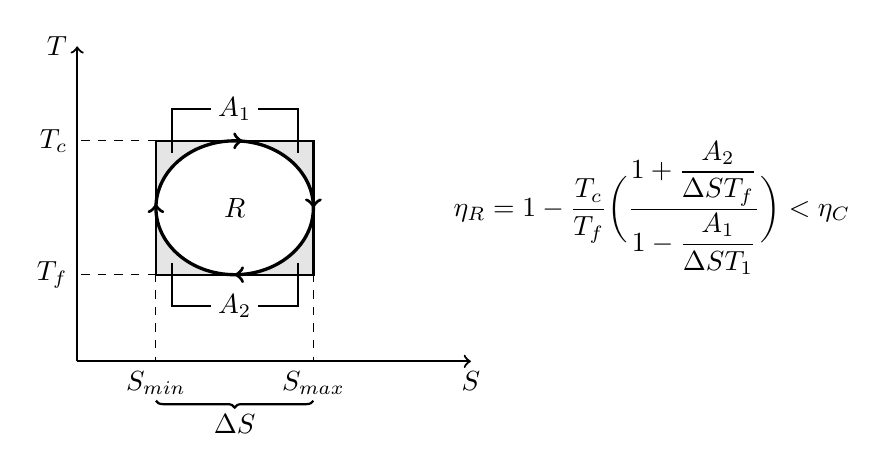
\begin{tikzpicture}
\draw[thick, ->] (-2,0) -- (3,0) node[anchor=north]{$S$};

\draw[thick, ->] (-2,0) -- (-2,4) node[anchor=east]{$T$};
\draw[thick] (-1,1.1) -- (-1,2.8) -- (1,2.8) -- (1,1.1) -- (-1,1.1);
\draw[thick, fill=black, fill opacity = 0.1] (-1,2.8) rectangle(1, 1.1);
\draw [very thick, fill=white] (0,1.95) ellipse (1 and 0.85) node[anchor=center] {$R$};
\draw [very thick, ->] (-1, 1.95) -- (-1,2);
\draw [very thick, ->] (1, 2) -- (1,1.95);
\draw [very thick, ->] (0, 2.8) -- (0.1,2.8);
\draw [very thick, ->] (0.1, 1.1) -- (0,1.1);
\draw[dashed] (-1,2.8) -- (-2, 2.8) node[anchor=east]{$T_c$};
\draw[dashed] (-1,1.1) -- (-2, 1.1) node[anchor=east]{$T_f$};
\draw[dashed] (-1,2.8) -- (-1, 0) node[anchor=north]{$S_{min}$};
\draw[dashed] (1,2.8) -- (1, 0) node[anchor=north]{$S_{max}$};
\draw[thick] (-0.8, 2.65) -- (-0.8, 3.2) -- (-0.3,3.2);
\draw[thick] (0.8, 2.65) -- (0.8, 3.2) -- (0.3,3.2);
\node[draw opacity = 0] at (0, 3.2) {$A_1$};
\draw[thick] (-0.8, 1.25) -- (-0.8, 0.7) -- (-0.3,0.7);
\draw[thick] (0.8, 1.25) -- (0.8, 0.7) -- (0.3,0.7);
\node[draw opacity = 0] at (0, 0.7) {$A_2$};
\draw[thick, decorate, decoration = {brace, mirror}] (-1, -0.5) -- (1, -0.5); 
\node[draw opacity = 0] at (0, -0.8){$\Delta S$};
\node at ( 5.3, 1.95){$\displaystyle \eta_R = 1 - \frac{T_c}{T_f}\bigg(\frac{\displaystyle 1 + \frac{A_2}{\Delta S T_f}}{\displaystyle  1 - \frac{A_1}{\Delta S T_1}}\bigg) < \eta_C$};
\end{tikzpicture}
\vspace{-0.5cm}
\end{figure}
\begin{description}
\item[Degradazione dell'energia] x bitermica irr. $\displaystyle \eta_{CLAUSIUS} \equiv \frac{\Delta S_U T_f}{Q_c}$ $\rightarrow$ $\boxed{\eta_M = \eta_C - \eta_{CLAUSIUS}}$ \\(MdC operante con stessi serb)
\\Politermica irreversibile $\eta_M = \eta_R - \eta_{CLAUSIUS} < \eta_C - \eta_{CLAUSIUS}$ con $R$ operante con medesimi serb. e $C$ con i due estremi 
\item[PRINCIPIO DI DEGRADAZIONE DELL'ENERGIA] in processo irreversibile $\boxed{\displaystyle L_{lost} = T_0 \cdot \Delta S_U}$ con $T_0$ temperatura termostato più freddo con cui sist. a contatto
\\Rev $\Delta S_U = 0 \, \implies$ massimo lavoro ottenibile
\item[Calore irrecuperabile] accoppiando irreversibile con frigo di Carnot $\displaystyle \overline{C}$ (max efficienza-rendimento): \\recuperabile $\displaystyle Q_c^{\overline{C}} = Q_c^M - \frac{T_c \, T_f}{T_c - T_f}\Delta S_U < Q_c^M$
\end{description}
\framebox{
\parbox{\linewidth}{
\vspace{0.1cm}
\textbf{RELAZIONE FONDAMENTALE DELLA TERMODINAMICA} per qualsiasi trasformazione ($U, S, V$ funzioni di stato | e lavoro qs rev)
\[\mathrm{d}U = T \mathrm{d}S - p \mathrm{d}V + \sum x_i \mathrm{d}X_i\]
con la sommatoria dei lavori termodinamici delle altre forze generalizzate. $\rightarrow S, V$ variabili naturali per $U$
}
}
\begin{description}
\item[GP con pistone a contatto termico con acqua] $\displaystyle T_f = T_0 \cdot 3^{\displaystyle \frac{R}{\mathcal{c}_V + C/n}}$ con $C$ capacità di acqua+contenitori
\[L_{est} = \frac{T_0}{n \mathcal{c}_V + C} \bigg(1 - 3^{\displaystyle \frac{R}{\mathcal{c}_V + C/n}}\bigg) \quad \Delta S_G = \frac{(1-\gamma) C \ln 3}{1 + C/(n \mathcal{c}_V)} \quad \Delta S_U = 0\]
\item[GP + vapor d'acqua saturo] compr isot rev. $\displaystyle p_f = p_0 \frac{V_0}{V_f} + p^\ast \bigg(1 - \frac{V_0}{V_f}\bigg)$ \hfill \bigg| \hfill $\displaystyle L = p^\ast (V_f - V_0) + (p_0 - p^\ast) V_0 \ln \frac{V_f}{V_0}$ con $p^\ast$ press di vap saturo. $\displaystyle m_{cond} = \mathcal{M} \Delta n_v = - \frac{\mathcal{M} p^\ast}{RT} (V_f - V_0)$
\item[2 S a contatto termico con capacità] $\displaystyle C(T) = \beta T$ \hfill \bigg\rangle \hfill $\displaystyle T_e = \sqrt{\frac{T_A^2 + T_B^2}{2}}$ \hfill \bigg| \hfill $\displaystyle \Delta S = \beta (2 T_e - T_A - T_B)$
\item[Massima temperatura con corpi in bagno termico] $T_0$ corpi, $T_B$ bagno. Usando MdC invertita 
\\$\displaystyle T_{max} = T_B + \sqrt{2} |T_0 - T_B|$ (analogo sia per $T_0 > T_B$ che viceversa)
\item[Serbatoio caldo = GP compresso a T cost] (MdC) $\quad \displaystyle \bigg(\frac{V_f}{V_i}\bigg)_{ciclo} = e^{\displaystyle \frac{L}{nR (T_c - T_f)}}$
\end{description}
\begin{minipage}{0.32\textwidth}
\centering
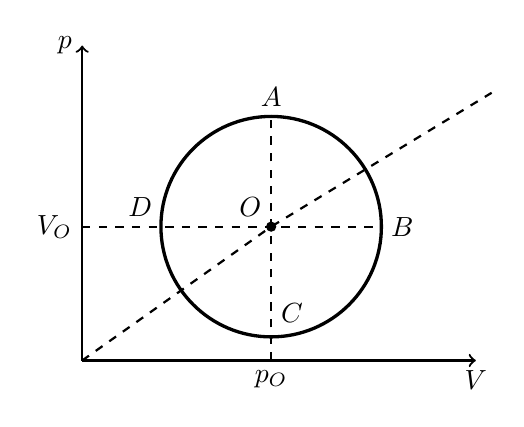
\begin{tikzpicture}
\draw[thick, ->] (-2,0) -- (3,0) node[anchor=north]{$V$};
\draw[very thick] (0.4,1.7) circle(1.4);

\draw[thick, fill=black](0.4, 1.7) circle(0.05) node[anchor=south]{$O \quad \enspace $};

\node[draw opacity = 0, anchor=south] at (0.4, 0.36){$\quad \enspace  C$};
\node[draw opacity = 0, anchor=south] at (0.4, 3.1){$A$};
\node[draw opacity = 0, anchor=south] at (-1, 1.7){$D \quad \enspace $};
\node[draw opacity = 0, anchor=west] at (1.8, 1.7){$B$};
\draw[thick, ->] (-2,0) -- (-2,4) node[anchor=east]{$p$};
\draw[dashed, thick] (0.4, 0)node[anchor=north]{$p_O$} -- (0.4,3.1);
\draw[dashed, thick] (-2,1.7)node[anchor=east]{$V_O$} -- (1.8, 1.7);
\draw[dashed, thick] (-2, 0) -- (0.4, 1.7) -- (3.2, 3.4);
\end{tikzpicture}
\end{minipage}
\begin{minipage}{0.68\textwidth}
\begin{description}
\item[Ciclo circolare] $\displaystyle \Delta U_{AC} = \frac{5}{2} V_A (p_C - p_A)$ \hfill \bigg| \hfill $\displaystyle L_{tot} = \pi \cdot (p_A - p_O) \cdot (V_B - V_O)$
\\Imponendo $\dd[•]{T} = 0$ si ha $\displaystyle \frac{p}{V} = \frac{p_O}{V_O}$ (giacciono su retta)
\\$\displaystyle Q_{ass} = \Delta U_{DB} + L_{DB} = \frac{L_{tot}}{2} + \frac{\gamma}{\gamma - 1} p_O (V_B - V_D)$ \hfill \bigg\rangle \hfill $\displaystyle \eta = \frac{L_{tot}}{Q_{ass}}$
\end{description}
\end{minipage}
\linebreak
\begin{minipage}{0.5\textwidth}
\begin{description}
\item[Ciclo peculiare GP] per $V_A, V_B$ si impone $p(V) = 2 p_0$
\[T_B = 3 T_0 \quad \big| \quad \displaystyle T_A = T_0\]
\[Q_{AB} = \frac{2 \gamma}{\gamma - 1} p_0 V_0  \quad \big\rangle \quad \textrm{ per mono: } \, Q_{AB}  = 5 p_0 V_0\]
\[L_{tot} = p_A (V_B - V_A) - \int_{A}^{B}p(V)\mathrm{d}V = \frac{2}{3} p_0 V_0 \quad \big\rangle \]
\[\big\rangle \quad Q_{BCA} = - \frac{13}{3} p_0 V_0 \quad \big| \quad \Delta S_{B \rightarrow C} = nR \ln \bigg( \frac{2}{\sqrt{243}} \bigg)\]
\end{description}
\end{minipage}
\begin{minipage}{0.5\textwidth}
\hfill
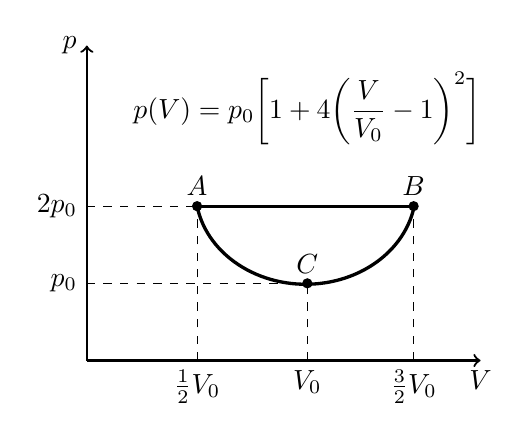
\begin{tikzpicture}
\node at (0.8, 3.2){$\displaystyle p(V) = p_0 \bigg[1 + 4 \bigg(\frac{V}{V_0} - 1\bigg)^2\bigg]$};
\draw[thick, ->] (-2,0) -- (3,0) node[anchor=north]{$V$};
\draw[thick, ->] (-2,0) -- (-2,4) node[anchor=east]{$p$};
\draw[very thick] (-0.6, 1.96) arc(-170:-10:1.4 and 1.2);
\draw[very thick] (-0.615, 1.96) -- (2.175, 1.96);
\draw[thick, fill=black](-0.6, 1.96) circle(0.05) node[anchor=south]{$A$};
\draw[thick, fill=black](2.15, 1.96) circle(0.05) node[anchor=south]{$B$};
\draw[thick, fill=black](0.8, 0.98) circle(0.05) node[anchor=south]{$C$};
\draw[dashed] (-2, 0.98)node[anchor=east]{$p_0$} -- (0.8,0.98);
\draw[dashed] (0.8, 0)node[anchor=north]{$V_0$} -- (0.8,0.98);
\draw[dashed] (-2, 1.96)node[anchor=east]{$2 p_0$} -- (-0.6, 1.96);
\draw[dashed] (2.15, 0)node[anchor=north]{$\frac{3}{2} V_0$} -- (2.15,1.96);
\draw[dashed] (-0.6, 0)node[anchor=north]{$\frac{1}{2} V_0$} -- (-0.6,1.96);


\end{tikzpicture}
\end{minipage}

\section{Potenziali termodinamici}
\begin{description}
\item[Entalpia] $\displaystyle H \equiv U + pV$ \bigg| $\displaystyle \mathrm{d}H = T\mathrm{d}S + V \mathrm{d}p$ ($S, \, p$ var nat)
\\A $p$ costante $\mathrm{d}H = (\delta Q_R)_p$
\item[Energia libera di Helmholtz] $\displaystyle F \equiv U - TS$ \bigg| $\displaystyle \mathrm{d}H = •\mathrm{d}U - T\mathrm{d}S - s\mathrm{d}T$ ($T, \, V$ var nat)
\\A $T$ cost $\displaystyle \mathrm{d}F = •\mathrm{d}U - T\mathrm{d}S \leq - \delta L$. In assenza di lavoro di volume $\displaystyle \mathrm{d}F \leq - \delta L^{(non-pV)}$
\item[Potenziali chimici] $\displaystyle \mu_i \equiv \bigg(\frac{\partial F}{\partial n_i}\bigg)_{T,V}$
\item[Equilibrio liquido-vapore] $\displaystyle \mathrm{d}F = 0$, $\displaystyle \mathrm{d}n_L = - \mathrm{d}n_G \implies \displaystyle \mu_L = \mu_G$
\item[Energia libera di Gibbs] $\displaystyle G \equiv H -TS = U -TS + pV$ \bigg| $\displaystyle \mathrm{d}G = V\mathrm{d}p - S\mathrm{d}T$ ($p, \, T$ var nat)
\\A $T$, $p$ cost $\displaystyle \mathrm{d}G \leq - \delta L^{(non-pV)}$
\item[In transizioni di fase] (sola specie!!) all'eq. $\displaystyle \frac{\partial^{•} G}{\partial n_i^{•}} = \mu_i = g_i \equiv \frac{G_i}{n_i}$ per ogni fase
\item[Gibbs per GP] $\displaystyle G(T,p) = RT\big[\Phi(T) + \ln \, p\big]$ con $\displaystyle \Phi(T) = (H_0 - TS_0 + \mathcal{c}_p T - \mathcal{c}_p T \, \ln T)/RT$
\\Per isoterme $\displaystyle \Delta G = \ln \frac{p_f}{p_i}$
\item[Gibbs per miscele di GP] $\displaystyle \mu_i(T,p) = g_i(T,p) + RT \,\ln x_i$ ove $x_i$ = fraz. molare (unica specie $\rightarrow$ caso prec)

\end{description}
\framebox{
\parbox{\linewidth}{
\vspace{0.1cm}
\textbf{RELAZIONI DI MAXWELL}
\\~\\ \textbf{I $\rangle$} $\displaystyle \bigg(\frac{\partial T}{\partial V}\bigg)_S = - \bigg(\frac{\partial p}{\partial S}\bigg)_V$ \hfill \textbf{II $\rangle$} $\displaystyle \bigg(\frac{\partial p}{\partial T}\bigg)_V = \bigg(\frac{\partial S}{\partial V}\bigg)_T$ 
\hfill \textbf{III $\rangle$} $\displaystyle \bigg(\frac{\partial T}{\partial p}\bigg)_S = \bigg(\frac{\partial V}{\partial S}\bigg)_p$ \hfill \textbf{IV $\rangle$} $\displaystyle \bigg(\frac{\partial V}{\partial T}\bigg)_p = - \bigg(\frac{\partial S}{\partial p}\bigg)_T$
\vspace{0.1cm}
}
}
{}
\\~\\\framebox{
\parbox{\linewidth}{
\vspace{0.1cm}
\textbf{EQUAZIONI DELL'ENERGIA}
\\ \begin{center}
\textbf{I $\rangle$} $\displaystyle \bigg(\frac{\partial U}{\partial V}\bigg)_T = T \bigg(\frac{\partial p}{\partial T}\bigg)_V - p$ \hspace{2cm} \textbf{II $\rangle$} $\displaystyle \bigg(\frac{\partial U}{\partial p}\bigg)_T = - T \bigg(\frac{\partial V}{\partial T}\bigg)_p - p \bigg(\frac{\partial V}{\partial p}\bigg)_T$
\end{center} 
\vspace{0.1cm}
}
}
\begin{description}
\item[Equazioni di Clapeyron] $\displaystyle \frac{\mathrm{d}^{•} p}{\mathrm{d}T^{•}} = \frac{\Delta \mathrm{v}}{\Delta \mathrm{v}•} = \frac{\lambda}{T \Delta \mathrm{v}}$ per passaggi di stato
\\Per temperature lontane da $T_c$, dunque $\mathrm{v}_G \gg \mathrm{v}_L \rightarrow \, \Delta \mathrm{v} \approx \mathrm{v}_G$ si ha $\boxed{\displaystyle p(T) = p_0 \, e^{\displaystyle - \frac{\lambda}{R} \big( \frac{1}{T} - \frac{1}{T_0}\big)}}$
\end{description}
\section{Terzo principio}
\begin{description}
\item[Principio di Nernst] $\displaystyle \lim\limits_{T \rightarrow 0} S(T, x_i) - S(T, x_f) = \Delta S = 0$ isoterma con $x$ coord term generica
\item[Enunciato di Planck] $\displaystyle S_0 = S(0) = 0$ per cristallo perfetto
\end{description}

\section{Termodinamica statistica}
\begin{description}
\item[Molteplicità di un macrostato] con $N$ particelle e $\mu$ cellette fisiche
\[W = \frac{N!}{\displaystyle \prod_{i=1}^\mu N_i!}\]
Sommando sui macrostati $\displaystyle \sum W = \mu^N$ e ovviamente $\displaystyle \sum\limits_{i=1}^\mu N_i = N$
\item[Volume in emispazio dello SdF] $\displaystyle \tau = W \Delta \tau$ con $\Delta \tau = (\Delta V)^N$ celletta in SdF e $\displaystyle \Delta V = \frac{V_{sist}}{\mu}$
\item[Quantizzazione SdF] $\displaystyle \mathrm{d}\vec{p} \, \mathrm{d}\vec{x} = \big(\frac{h}{4\pi}\big)^{3N}$
\end{description}
\framebox{
\parbox{\linewidth}{
\vspace{0.1cm}
\textbf{ENTROPIA DI BOLTZMANN}
\[S = k_B \ln W\]
}
}
\begin{description}
\item[Funzione di partizione] $\displaystyle Z = \sum e^{- \beta \varepsilon_i}$ con $\displaystyle \beta = \frac{1}{k_B T}$
\item[Distribuzione di Boltzmann] $\displaystyle p_i(\varepsilon_i) = \frac{e^{-\varepsilon_i/k_B T}}{Z}$
\item[Ricavare funz termodinamiche] $\displaystyle U = - N \frac{\partial^{} \ln Z}{\partial \beta^{•}}$ \bigg| $\displaystyle \langle \varepsilon \rangle = - \frac{\partial^{•} \ln Z}{\partial \beta^{•}}$
\item[Informazione] $\displaystyle I_i = I(x_i) = - \log_b p_i$ con $x_i$ possibile outcome di variabile aleatoria discreta con probabilità $p_i$.
\item[\large ENTROPIA DI SHANNON] $\displaystyle S_I \equiv \sum p_i I(x_i) = - \sum p_i \, \log_b p_i = - k_I \sum p_i \, \ln p_i$ con $\displaystyle k_I \equiv \frac{1}{\ln b}$
\end{description}

\section{Differenziali esatti}
Funzionale (1-forma su spazio vettoriale) in due coordinate generiche:
\[\alpha = a(x,y) \mathrm{d}x + b(x,y) \mathrm{d}y\]
Se $\exists \, Q$ : $\displaystyle a = \pdv[•]{Q}{x}$ e $\displaystyle b = \pdv[•]{Q}{y}$ allora $\alpha = \mathrm{d}Q$ differenziale esatto, dunque integrabile con $\displaystyle Q = \int \alpha = \int (\vec{\grad} Q) \cdot \mathrm{d}\vec{x}$
\\~\\Ciò è verificato \textbf{se e solo se} $a,b$ definite su insieme \textit{semplicemente connesso} e vale il \textbf{Teorema di Schwarz}, ovvero:
\[\pdv[]{Q}{x}{y} = \pdv[•]{a}{y} = \pdv[]{Q}{y}{x} = \pdv[•]{b}{x}\]
\newpage 
\section{Costanti fisiche, u.m. e proprietà termodinamiche}
\subsection*{Costanti e u.m.}
\paragraph{Costanti}
\begin{description}
\item[Velocità della luce nel vuoto] $\displaystyle c = 299792458 \, \mathrm{m \, s^{-1}}$
\item[Costante di Gravitazione universale] $\displaystyle G = 6.67428 \times 10^{-11} \, \mathrm{N \, m^2 \, kg^{-2}}$
\item[Accelerazione di gravità] (in prossimità del suolo) $\displaystyle g \approx 9.81 \, \mathrm{m \, s^{-2}}$
\item[Costante dei Gas] $\displaystyle R = 8.314472 \, \mathrm{J \, mol^{-1} \, K^{-1}}$
\item[Numero di Avogadro] $\displaystyle N_A \approx 6.02214179 \times 10^{23} \, \mathrm{mol^{-1}}$
\item[Costante di Boltzmann] $\displaystyle k_B \equiv \frac{R}{N_A} \approx 1.3806504 \times 10^{23} \, \mathrm{J \, K^{-1}}$ 
\item[Costante di Planck] $\displaystyle h \approx 6.62606896 \times 10^{-34} \, \mathrm{J \, s}$
\item[Costante di Stefan-Boltzmann] $\displaystyle \sigma \approx 5.670367 \times 10^{-8} \, \mathrm{W \, m^{-2} \, K^{-4}}$
\item[Costante dello spostamento di Wien] $\displaystyle b = 2.9 \times 10^{-3} \, \mathrm{m \, K}$
\end{description}
\paragraph{Unità di misura}
\[1 \, \mathrm{eV} = 1.6 \times 10^{-19} \, \mathrm{J} = 1.16 \times 10^{4} \, \mathrm{K}\]
\[1 \, \mathrm{\AA} = 10^{-10} \, \mathrm{m}\]
\[1 \, \mathrm{atm} = 1.01325 \times 10^{5} \, \mathrm{Pa}\]
\[1 \, \mathrm{bar} = 10^{5} \, \mathrm{Pa}\]
\[1 \, \mathrm{mmHg} = 133.3 \, \mathrm{Pa}\]
\[1 \, \mathrm{cal} = 4.18 \, \mathrm{J}\]

\paragraph{Condizioni peculiari}
\begin{itemize}
\item Condizioni standard (STP) \dotfill $ 0 \, \mathrm{{}^\circ C} \enspace \big| \enspace 10^5 \, \mathrm{Pa}$
\item Condizioni normali \dotfill $ 300 \, \mathrm{K} \enspace \big| \enspace 1 \, \mathrm{atm}$

\end{itemize}

\subsection*{Proprietà termodinamiche}
\paragraph{Densità}
\begin{itemize}
\item Ghiaccio \dotfill $ 917 \, \mathrm{kg \, m^{-3}}$
\item Acqua distillata \dotfill $ 1000 \, \mathrm{kg \, m^{-3}}$
\end{itemize}
\paragraph{Temperatura di punto triplo ($T_3$)}
\begin{itemize}
\item Acqua \dotfill $273.16 \, \mathrm{K} \, \big/ \, 0.01 \, \mathrm{{}^{\circ} C}$
\item Ossigeno \dotfill $54.36 \, \mathrm{K} \, \big/ \, -218.79 \, \mathrm{{}^{\circ} C}$
\item Idrogeno \dotfill $13.80 \, \mathrm{K} \, \big/ \, -259.35 \, \mathrm{{}^{\circ} C}$
\item Mercurio \hfill $234.32 \, \mathrm{K} \, \big/ \, -38.83 \, \mathrm{{}^{\circ} C}$
\end{itemize}
\paragraph{Punto di solidificazione / fusione}
\begin{itemize}
\item Alluminio \dotfill $933.47 \, \mathrm{K} \, \big/ \, 660.32 \, \mathrm{{}^{\circ} C}$
\item Oro \dotfill $1337.33 \, \mathrm{K} \, \big/ \, 1064.18 \, \mathrm{{}^{\circ} C}$
\item Rame \dotfill $1357.77 \, \mathrm{K} \, \big/ \, 1084.62 \, \mathrm{{}^{\circ} C}$
\end{itemize}
\paragraph{Calori latenti per acqua}
\begin{itemize}
\item Fusione \dotfill $ 333 \, \mathrm{J \, g^{-1}}$
\item Vaporizzazione \dotfill $ 2272 \, \mathrm{J \, g^{-1}}$
\end{itemize}
\paragraph{Calore specifico (per unità di massa)}
\begin{itemize}
\item Ghiaccio \dotfill $ 2.05 \, \mathrm{J \, g^{-1} K^{-1}}$
\item Acqua \dotfill $ 4.18 \, \mathrm{J \, g^{-1} K^{-1}}$
\item Vapore \dotfill $ 2.08 \, \mathrm{J \, g^{-1} K^{-1}}$
\item Alluminio \dotfill $ 0.88 \, \mathrm{J \, g^{-1} K^{-1}}$
\end{itemize}
\paragraph{Coefficiente di dilatazione lineare ($\alpha_L$)}
\begin{itemize}
\item Acciaio \dotfill $1.2 \times 10^{-5} \, \mathrm{K^{-1}}$
\item Alluminio \dotfill $2.4 \times 10^{-5} \, \mathrm{K^{-1}}$
\item Platino \dotfill $9 \times 10^{-6} \, \mathrm{K^{-1}}$
\end{itemize}
\paragraph{Coefficiente di dilatazione volumetrico ($\alpha$)}
\begin{itemize}
\item Ghiaccio \dotfill $1.5 \times 10^{-4} \, \mathrm{K^{-1}}$
\item Aria \dotfill $3.4 \times 10^{-3} \, \mathrm{K^{-1}}$
\item Vetro \dotfill $-3 \times 10^{-5} \, \mathrm{K^{-1}}$
\item Mercurio \dotfill $1.8 \times 10^{-4}\, \mathrm{K^{-1}}$
\end{itemize}
\paragraph{Coefficiente di comprimibilità isoterma ($k$)}
\begin{itemize}
\item Acqua \dotfill $2.2 \, \mathrm{GPa}$
\item Aria \dotfill $10^{5} \, \mathrm{Pa}$
\item Acciaio \dotfill $ 160 \, \mathrm{GPa}$ 
\item Diamante \dotfill $400 \, \mathrm{GPa}$
\end{itemize}
\paragraph{Costanti di Van der Waals}
\begin{itemize}
\item Anidride carbonica \dotfill $a = 364 \, \mathrm{L^2 \, kPa \, mol^{-2}} \quad \big/ \quad b = 0.043 \, \mathrm{L \, mol^{-1}}$ 
\item Ossigeno \dotfill $a = 138 \, \mathrm{L^2 \, kPa \, mol^{-2}} \quad \big/ \quad b = 0.032 \, \mathrm{L \, mol^{-1}}$ 
\item Vapore acqueo \dotfill $a = 553 \, \mathrm{L^2 \, kPa \, mol^{-2}} \quad \big/ \quad b = 0.030 \, \mathrm{L \, mol^{-1}}$ 
\item Etanolo \dotfill $a = 1218 \, \mathrm{L^2 \, kPa \, mol^{-2}} \quad \big/ \quad b = 0.084 \, \mathrm{L \, mol^{-1}}$ 
\item Azoto ($N_2$) \dotfill $a = 141 \, \mathrm{L^2 \, kPa \, mol^{-2}} \quad \big/ \quad b = 0.039 \, \mathrm{L \, mol^{-1}}$ 
\end{itemize}
\paragraph{Diametro molecolare}
\begin{itemize}
\item Ossigeno, azoto ($O_2$, $N_2$) \dotfill $ 1.7 \, \mathrm{\AA}$ 
\end{itemize}
\paragraph{Massa molecolare}
\begin{itemize}
\item Aria \dotfill $ 28.8 \, \mathrm{uma}$
\end{itemize}
\paragraph{Energie molecolari per l'acqua}
\begin{itemize}
\item Legame a idrogeno \dotfill $ 0.2 \, \mathrm{eV}$
\item Energia cinetica media \dotfill $ 0.04 \, \mathrm{eV}$
\item Minimo potenziale LJ \dotfill $ 0.03 \, \mathrm{eV}$

\end{itemize}
\paragraph{Velocità medie molecolari a 300 K} come $\displaystyle \sqrt{\langle v^2 \rangle}$
\begin{itemize}
\item Idrogeno ($H_2$) \dotfill $ 1934 \, \mathrm{m \, s^{-1}}$ 
\item Azoto ($N_2$) \dotfill $ 493 \, \mathrm{m \, s^{-1}}$ 
\end{itemize}
\paragraph{Libero cammino medio a 300 K e 1 atm}
\begin{itemize}
\item Ossigeno, azoto ($O_2$, $N_2$) \dotfill $ 320 \, \mathrm{nm}$ 
\end{itemize}
\paragraph{Conducibilità termica}
\begin{itemize}
\item Argento, Rame \dotfill $ 400 \, \mathrm{W \, m^{-1} \, K^{-1}}$ 

\item Ghiaccio \dotfill $ 2 \, \mathrm{W \, m^{-1} \, K^{-1}}$ 

\item Vetro \dotfill $ 1 \, \mathrm{W \, m^{-1} \, K^{-1}}$ 

\item Aria \dotfill $ 0.02 \, \mathrm{W \, m^{-1} \, K^{-1}}$ 
\end{itemize}

\paragraph{Irraggiamento solare}
\begin{itemize}
\item Costante solare (in cima all'atmosfera) $k_s$ \dotfill $ 1350 \, \mathrm{W \, m^{-2}}$ 
\item Costante solare (al suolo) $k_s'$ \dotfill $ 1000 \, \mathrm{W \, m^{-2}}$ 
\item $\lambda_{max}$ spettro solare \dotfill $ 510 \, \mathrm{nm}$ 
\item Albedo medio (frazione luce riflessa) terrestre $a$ \dotfill $ 0.30$ 
\end{itemize}
\paragraph{Bilancio termico corpo umano}
\begin{itemize}
\item Superficie media \dotfill $ 1.5 \, \mathrm{m^2}$ 
\item Coefficiente di trasferimento termico ($h = h_{conv} + h_{rad}$) \dotfill $ 6.5 \, \mathrm{W \, m^{-2} \, K^{-1}}$ 
\item Valore ottimale temperatura esterna \dotfill $ 26 \, \mathrm{{}^\circ C}$ 
\end{itemize}
\paragraph{Dulong Petit}
\begin{itemize}
\item Costante di proporzionalità $A$ per $C(T) = A T^3$ nel limite $T \rightarrow 0$ \dotfill $ 1.25 \times 10^{-3} \, \mathrm{J \, kg^{-1} K^{-4}}$ 
\end{itemize}
\paragraph{Respirazione cellulare}
\begin{itemize}
\item $\Delta g$ molare \dotfill $ -2840 \, \mathrm{kJ \, mol^{-1}}$
\end{itemize}
\paragraph{Volumi molari per acqua a 300 K e 1 atm}
\begin{itemize}
\item Gassoso ($\mathrm{v}_G$) \dotfill $ 2.5 \times 10^{4} \, \mathrm{cm^{3}}$
\item Liquido ($\mathrm{v}_L$) \dotfill $ 18 \, \mathrm{cm^{3}}$
\end{itemize}


\end{document}